\documentclass[dvipdfm, aspectratio=169]{beamer}

\usepackage{bm}
\usepackage{
    amsmath,
    amsfonts
}
\usepackage{helvet}
\usepackage{listings}
\usepackage{xcolor}
\lstset{
  language={python},
  basicstyle={\ttfamily\tiny},
  keywordstyle={\color{blue}},
  commentstyle={\color{green}},
  stringstyle=\color{red},
  tabsize=2,
  breaklines=true,
}

\usetheme{Madrid}
\usecolortheme{crane}
\setbeamercolor{structure}{fg=orange}
\setbeamercolor{block title example}{fg=white}
\setbeamercolor{block title alerted}{fg=white}
\setbeamertemplate{navigation symbols}{}
\setbeamertemplate{blocks}[rounded][shadow=false]
\setbeamertemplate{items}[circle]
\renewcommand{\kanjifamilydefault}{\gtdefault}
\usefonttheme[onlymath]{serif}
\renewcommand{\figurename}{図}
\renewcommand{\tablename}{表}
\renewcommand{\footnoterule}{
  \hrule width \textwidth height 0.5pt
  \kern 4pt
}
\setbeamercolor{title}{fg=black}
\setbeamercolor{frametitle}{fg=black}
\setbeamercolor{block title}{fg=black}
\setbeamercolor{block title example}{fg=white}

\def\q{\bm{q}}
\def\k{\bm{k}}

\title[研究会]{
    Transformerモデルのコンテキスト拡張手法
}
\subtitle[]{情報数理システム分野 研究会}
\author[平田 蓮]{平田 蓮}
\date{2024年7月10日}

\begin{document}
    \begin{frame}
        \titlepage
    \end{frame}
    \begin{frame}{RoPE}
        \begin{itemize}
            \item 位置エンコーディングを加算ではなく乗算で行うアプローチ
            \item LLaMAなどで用いられており、現在主流である
            \item {
                QueryとKeyに回転行列をかけて、ベクトルを回転させることで位置情報を乗せる
            }
        \end{itemize}

        \begin{block}{RoPEの特徴}
            \begin{itemize}
                \item トークンの位置ごとに回転角を増やしていくため、絶対位置情報を反映可能
                \item 距離の近いトークンの回転角同士が成す角が小さいため、相対位置情報も反映可能
            \end{itemize}
        \end{block}

        回転行列は、トークンの位置$m$と埋め込みの次元$D$を用いて次のように表せる
    \end{frame}
    \begin{frame}{RoPE}
        \begin{block}{回転行列の計算}
            {\small
                \begin{align*}
                    R &= \begin{pmatrix}
                        \cos m\theta_1 & -\sin m\theta_1 & 0 & 0 & \cdots & 0 & 0 \\
                        \sin m\theta_1 & \cos m\theta_1 & 0 & 0 & \cdots & 0 & 0 \\
                        0 & 0 & \cos m\theta_2 & -\sin m\theta_2 & \cdots & 0 & 0 \\
                        0 & 0 & \sin m\theta_2 & \cos m\theta_2 & \cdots & 0 & 0 \\
                        \vdots & \vdots & \vdots & \vdots & \ddots & \vdots & \vdots \\
                        0 & 0 & 0 & 0 & \cdots & \cos m\theta_\frac{D}{2} & -\sin m\theta_\frac{D}{2} \\
                        0 & 0 & 0 & 0 & \cdots & \sin m\theta_\frac{D}{2} & \cos m\theta_\frac{D}{2}
                    \end{pmatrix} \\
                    \theta_i &= 10000^{-\frac{2(i-1)}{D}} \ \left(i = 1, 2, \cdots, \frac{D}{2}\right)
                \end{align*}
            }
        \end{block}
        これを用いて計算した$^t\!Q' = R{}^t\!Q, ^t\!K' = R{}^t\!K$により
        Attention行列を計算する。
    \end{frame}
    \begin{frame}{入力シーケンスの拡張}
        入力シーケンス(コンテキスト)長を拡張する手法として以下について述べる
        \begin{itemize}
            \item Position Interpolation
            \item YaRN
            \item LongNet
            \item LongLoRA
        \end{itemize}
    \end{frame}
    \begin{frame}{Position Interpolation}
        \begin{itemize}
            \item {Shouyuanらとkaiokendev
            によって提案されたRoPEのシンプルな拡張}
            \item{
                トークン位置を元のコンテキスト長と新しいコンテキスト長の比率を
                用いてスケールする
            }
        \end{itemize}

        \begin{block}{}
            RoPEの回転行列において、
            $m\rightarrow \frac{L}{L'}m$とする。
            \begin{description}
                \item[$L$] 元のコンテキスト長
                \item[$L'$] 拡張したコンテキスト長
            \end{description}
            $\frac{L'}{L}$をスケール倍率と呼ぶ。
        \end{block}

        \begin{itemize}
            \item{
                少数ショット学習を行うことで
                コンテキストを拡張できることが示された
            }
            \item{
                しかし、一定より高いスケール倍率を用いると、
                性能が低下する
            }
        \end{itemize}
    \end{frame}
    \begin{frame}{YaRN}
        \begin{block}{RoPEの波長}
            $d$次元目における回転角$\theta_d$を用いて波長$\lambda_d$を定義する
            \begin{align*}
                \lambda_d=\frac{2\pi}{\theta_d}
            \end{align*}

            波長は、その次元に対する位置エンコーディングの回転が一周するのに必要なトークン数
        \end{block}
        Bowenらは、この波長に着目し、
        RoPEのコンテキスト拡張を行った
    \end{frame}
    \begin{frame}{YaRN}
        埋め込みの高次元部分において、
        学習したコンテキスト長よりも波長が長い次元が存在する

        $\rightarrow$その次元においては位置エンコーディングが回転領域で均等に分布していない

        $\rightarrow$埋め込みが一回転しないため、Position Interpolationを行なっても\structure{絶対位置の情報が保存される}

        逆に、波長が短い次元においては、
        \structure{絶対位置の情報が消えてしまう}
    \end{frame}
    \begin{frame}{YaRN}
        さらに、Position Interpolationを高いスケール倍率で行うと性能が低下する

        $\rightarrow$スケール倍率を高くするほど距離が近いトークン同士の
        位置エンコーディングの差異が小さくなり、
        関係性をうまくモデルが認識できなくなっている
    \end{frame}
    \begin{frame}{YaRN}
        以上の仮定をもとに、Position Interpolationに次のような変更を行った
        \begin{itemize}
            \item $\lambda_d$が$L$に対して十分に小さい次元ではスケーリングを行わない
            \item $\lambda_d$が$L$以上の次元では、$L'=\lambda_d$としたスケーリングを行う
            \item 上二つの間の次元領域では、波長の長さに応じて回転角を調整する
        \end{itemize}
    \end{frame}
    \begin{frame}{YaRN}
        \begin{block}{}
            二つのハイパーパラメータ$\alpha,\beta$を用いて以下の式で表される
            \begin{align*}h(\theta_d, \lambda_d) &= \left(1-\gamma\left(\frac{L}{\lambda_d}\right)\right)\frac{L}{L'}\theta_d + \gamma\left(\frac{L}{\lambda_d}\right)\theta_d \\
                \gamma(r) &= \left\{ \begin{aligned}
                    &0 \ &(r < \alpha) \\
                    &1 \ &(r > \beta) \\
                    &\frac{r-\alpha}{\beta-\alpha} \ &(\mathrm{otherwise})
                \end{aligned}\right.
            \end{align*}
            Position Interpolationと違い、
            $\theta_d'=h(\theta_d,\lambda_d)$として、
            $m$ではなく回転角に対してスケーリングを行う
        \end{block}
        \begin{itemize}
            \item $r$は波長に対する元のコンテキスト長の比
            \item $\gamma$はこの比をもとにスケーリングする比率を計算する
        \end{itemize}
    \end{frame}
    \begin{frame}{実験結果}
            \begin{figure}[ht]
                \begin{center}
                    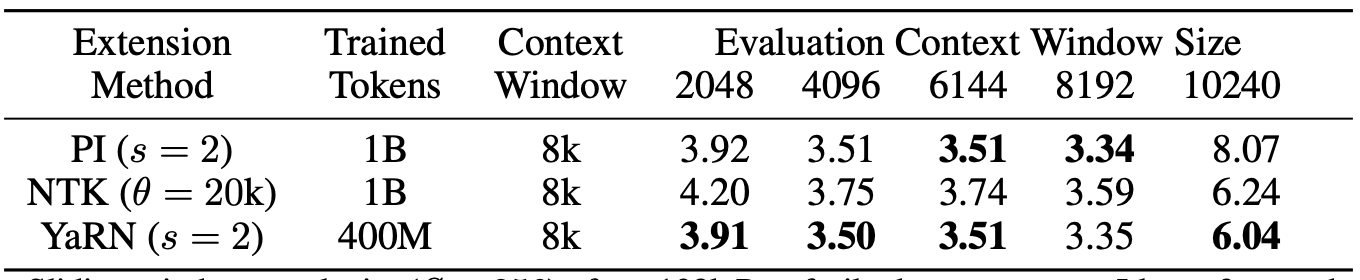
\includegraphics[width=.6\hsize]{yarn1.png}
                    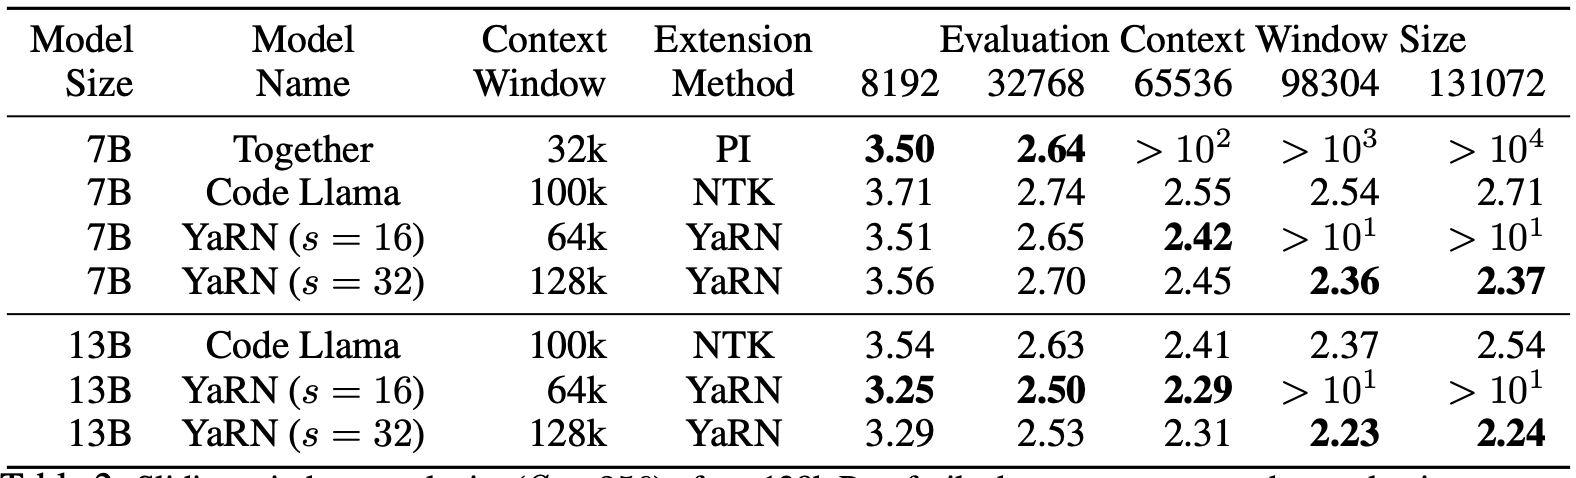
\includegraphics[width=.7\hsize]{yarn2.png}
                \end{center}
            \end{figure}

            \begin{itemize}
                \item 上の表では、各手法に対してYaRNが少ない学習量でも優位であることが示された
                \item 下の表では、YaRNが高いスケーリング倍率でも有効であることが示された
            \end{itemize}
    \end{frame}
    \begin{frame}{LongNet}
        \begin{itemize}
            \item Jiayuらによって提案されたモデル
            \item 後述するDialated Attentionという構造を用いて
            コンテキスト長を10億まで拡張できることを示した
        \end{itemize}
    \end{frame}
    \begin{frame}{Dialated Attention}
        \begin{itemize}
            \item{
                トークンのAttentionを計算する際に、
                入力を複数の大きさのブロックに分割する
            }
            \item{
                ブロックの大きさに応じて、
                Attentionを計算するトークンの間隔を広げ、
                一定の大きさの入力としている
            }
            \item{
                これらの結果を合算し、離れた位置にあるトークン同士の依存関係も捉えている
            }
        \end{itemize}
        \begin{figure}[ht]
            \centering
            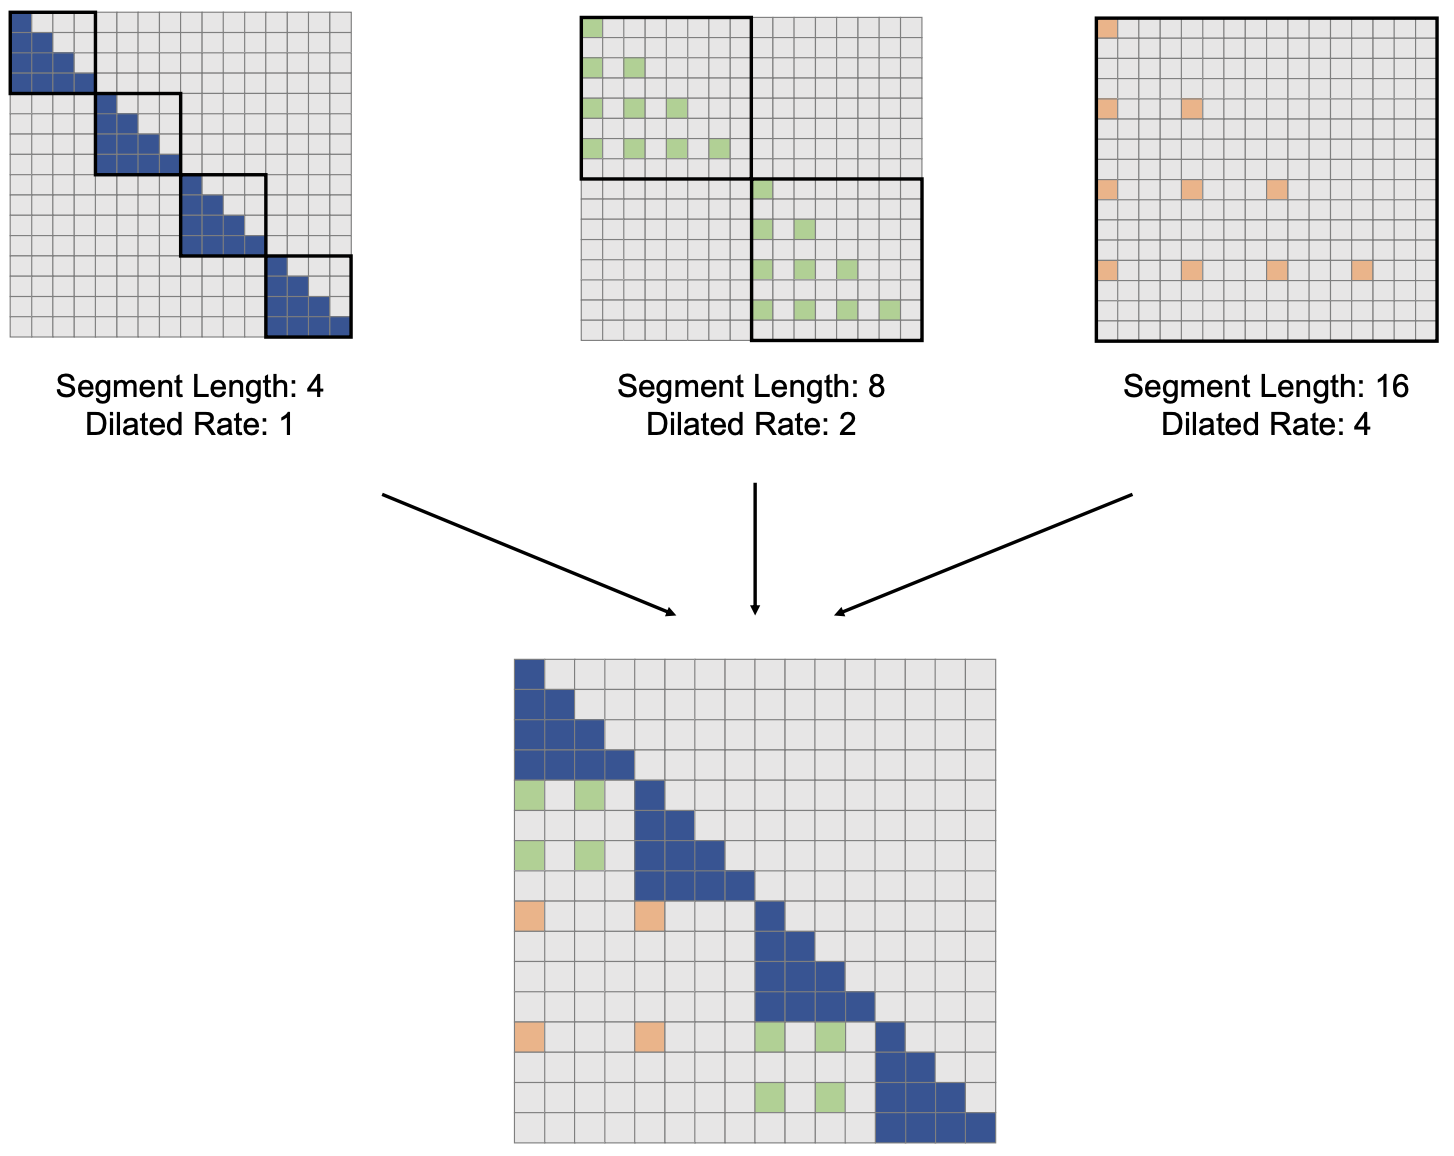
\includegraphics[width=.4\hsize]{dialated.png}
        \end{figure}
    \end{frame}
    \begin{frame}{Dialated Attention}
        さらに、各Attention headにおいてAttentionを計算するトークンのパターンを変更する

        $\rightarrow$すべてのトークン間の依存関係を捉えられる
        \begin{figure}[ht]
            \centering
            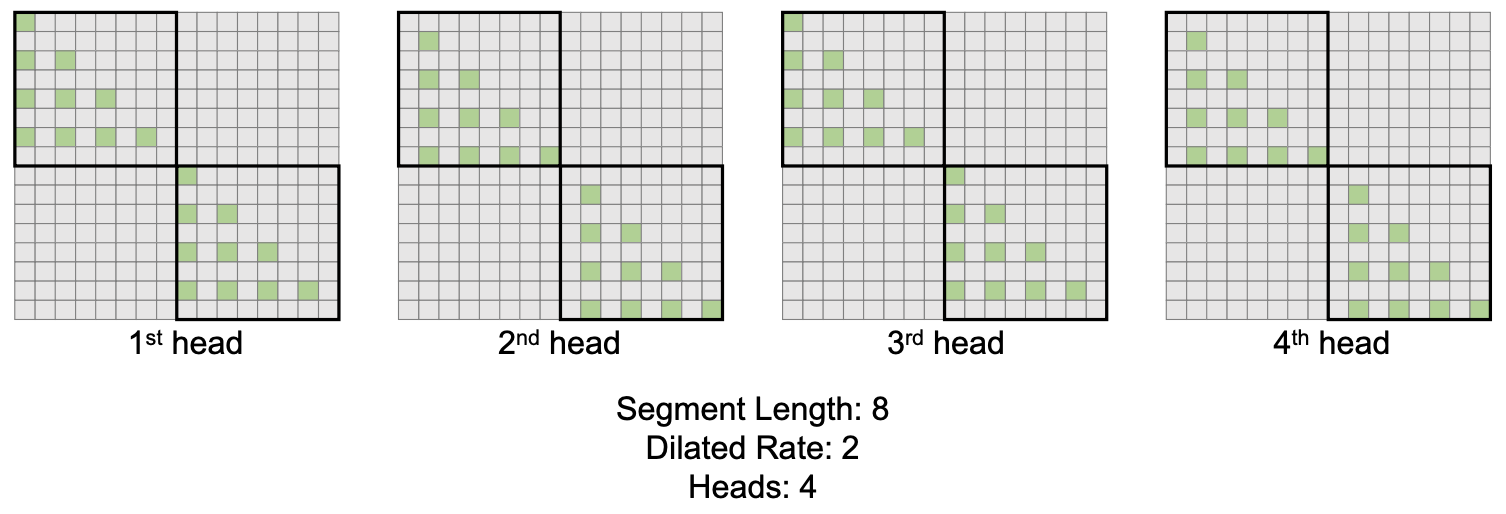
\includegraphics[width=.9\hsize]{dialated_pattern.png}
        \end{figure}
    \end{frame}
    \begin{frame}{実験結果}
        \begin{itemize}
            \item{
                Dialated Attentionに加え、
                時間計算量を抑える為に、
                分散アルゴリズムを用いてトークン長と埋め込み次元に対する
                線形時間で学習が行われた
            }
            \item{
                32kまでのコンテキスト長でベースのTransformerモデルと同様の性能を発揮するこが確認された
            }
            \item{
                さらにコンテキスト長を拡張しても性能が低下しないことが確認された
            }
        \end{itemize}
        以上より、コンテキスト長を10億まで拡張できると結論づけられた。

        \begin{figure}[ht]
            \centering
            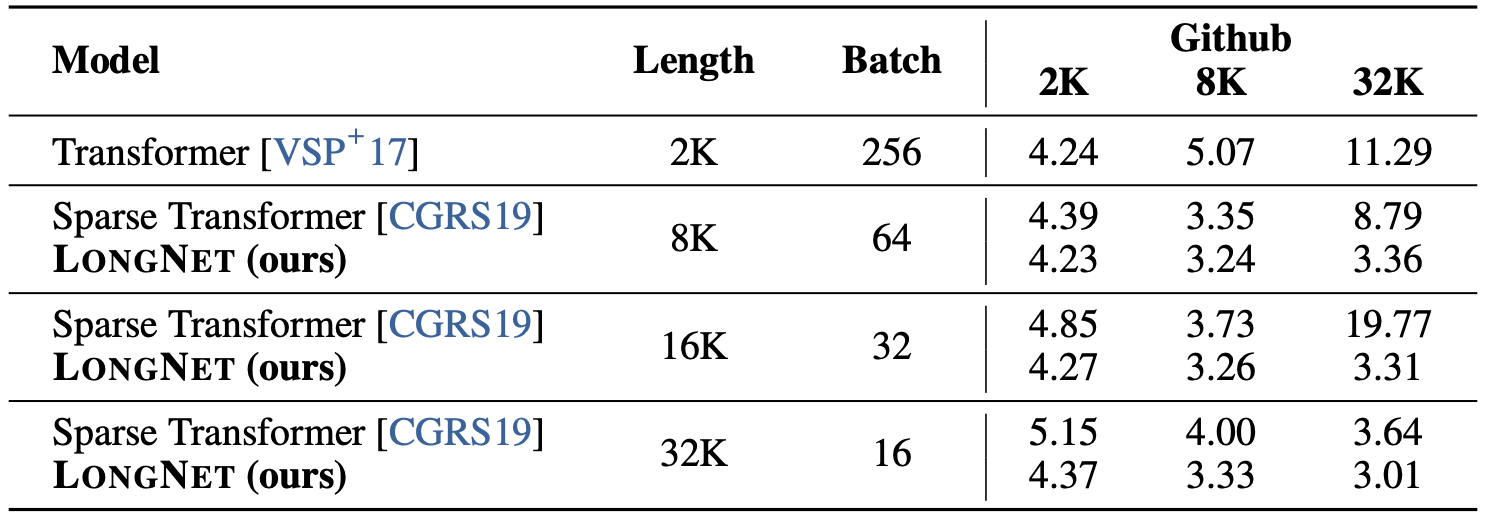
\includegraphics[width=.65\hsize]{longnet.png}
        \end{figure}
    \end{frame}
    \begin{frame}{LongLoRA}
        \begin{itemize}
            \item{
                Yukangらによって提案された、
                コンテキスト長が大きい場合でも効率的にLoRAを適用する手法
            }
            \item{
                Position Interpolationなどによってコンテキスト長を拡張した
                モデルに対してファインチューニングを行うことを仮定
            }
        \end{itemize}
        通常のLoRAではコンテキスト長が大きくなるにつれてperplexityが
        大きくなってしまう。
        一方、通常のファインチューニングは低いperplexityを維持するが、
        計算コストとVRAMの消費量が膨大になってしまう

        \begin{block}{}
            LongLoRAでは、後述のShifted Sparse Attentionを用いて、
            \begin{itemize}
                \item 通常のファインチューニングと同等のperplexity
                \item LoRAと同等のVRAM消費量
                \item 小さい計算量
            \end{itemize}
            でのファインチューニングを実現している
        \end{block}
    \end{frame}
    \begin{frame}{Shifted Sparse Attention}
        \begin{itemize}
            \item{
                入力シーケンスを分割し、
                分割したブロックごとにAttention機構に通す

                $\rightarrow$計算量が改善
            }
            \item{
                各ブロックの大きさの半分だけずらして分割をした入力を
                同様にAttention機構に通す
            }
            \item{
                これらのAttentionを合算することで、計算量を抑えつつ、
                ブロック間の依存関係を捉える
            }
        \end{itemize}
        \begin{figure}[ht]
            \centering
            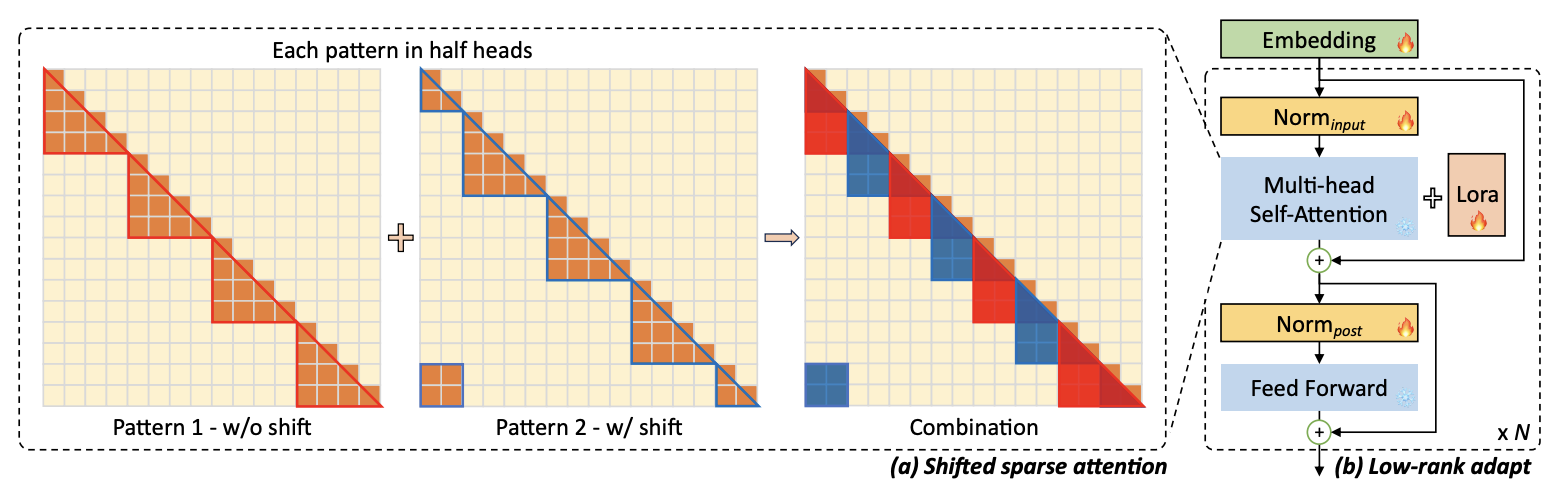
\includegraphics[width=.9\hsize]{ssa.png}
        \end{figure}
    \end{frame}
    \begin{frame}{実験結果}
        Perplexity、VRAM使用量、学習時間の三つの観点からLongLoRA
        の評価が行われた
        \begin{figure}[ht]
            \centering
            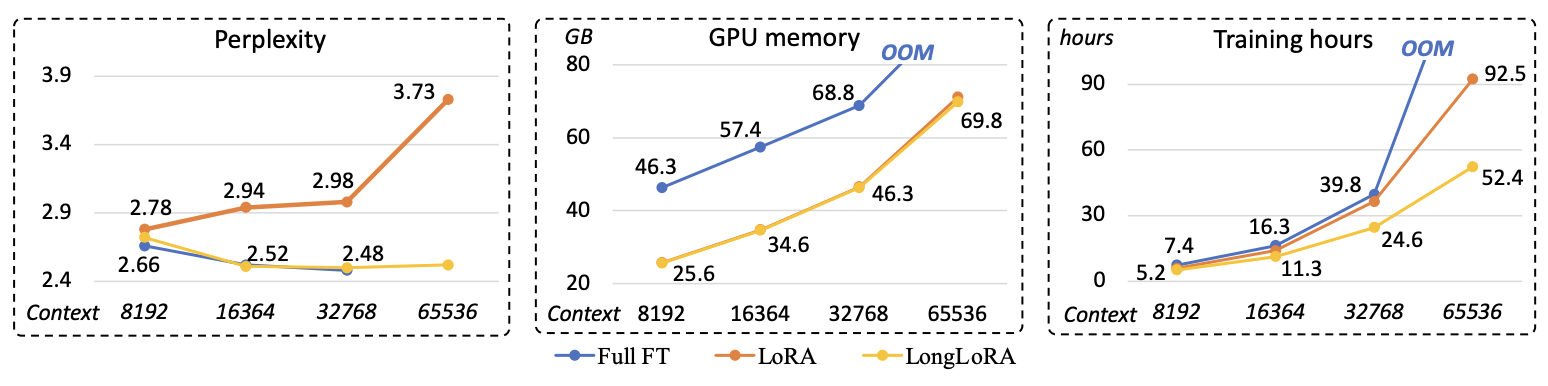
\includegraphics[width=\hsize]{longlora.png}
        \end{figure}

        通常のファインチューニングと同様の性能を維持しつつ、
        LoRAと同様にVRAM使用量を抑え、
        かつLoRAより少ない時間で学習できている
    \end{frame}
    \begin{frame}{外挿によるコンテキスト拡張}
        Yutaoらは外挿(学習データより長いシーケンスの入力)
        を可能にする手法を提案した

        \begin{block}{Attention Resolution}
            外挿能力の指標
            \begin{align*}
                R(s) = \sum_{i=0}^N\frac{e^{s[i]}\left(e^{s[i]}-e^{s[i+1]}\right)}{\left(\sum_{i=0}^Ne^{s[i]}\right)^2}
            \end{align*}
            \begin{description}
                \item[$s\textrm{[}i\textrm{]}$]{
                    距離が$i$のトークン間のAttentionスコア
                    (Attention行列の要素)の期待値
                }
            \end{description}
        \end{block}

        後述の2手法を用いてAttention Resolutionが増大された
    \end{frame}
    \begin{frame}{位置エンコーディングによるAttention Resolutionの増加}
        RoPEを改良した次の位置エンコーディング$f_q,f_k$を用いた
        \begin{block}{}
            {\small
            \begin{align*}
                f_q(\q,n) = \begin{pmatrix}
                    q_1\cos n\zeta^n_1\theta_1 - q_2\sin n\zeta_1^n\theta_1 \\
                    q_2\cos n\zeta^n_1\theta_1 + q_1\sin n\zeta_1^n\theta_1 \\
                    \vdots \\
                    q_{D-1}\cos n\zeta^n_{\frac{D}{2}}\theta_{\frac{D}{2}} - q_D\sin n\zeta^n_{\frac{D}{2}}\theta_{\frac{D}{2}} \\
                    q_D\cos n\zeta^n_{\frac{D}{2}}\theta_{\frac{D}{2}} + q_{D-1}\sin n\zeta^n_{\frac{D}{2}}\theta_{\frac{D}{2}}
                \end{pmatrix},f_k(\k,n) = \begin{pmatrix}
                    k_1\cos n\zeta^{-n}_1\theta_1 - k_2\sin n\zeta^{-n}_1\theta_1 \\
                    k_2\cos n\zeta^{-n}_1\theta_1 + k_1\sin n\zeta^{-n}_1\theta_1 \\
                    \vdots \\
                    k_{D-1}\cos n\zeta^{-n}_{\frac{D}{2}}\theta_{\frac{D}{2}} - k_D\sin n\zeta^{-n}_{\frac{D}{2}}\theta_{\frac{D}{2}} \\
                    k_D\cos n\zeta^{-n}_{\frac{D}{2}}\theta_{\frac{D}{2}} + k_{D-1}\sin n\zeta^{-n}_{\frac{D}{2}}\theta_{\frac{D}{2}}
                \end{pmatrix}
            \end{align*}
            }
            \begin{description}
                \item[$\q,\k$]{
                    あるトークンに対するQueryとKey:
                    $\q={}^t(q_1,\cdots,q_D), \k={}^t(k_1,\cdots,k_D)$
                }
                \item[$n$]{
                    トークンの位置
                }
            \end{description}
        \end{block}
    \end{frame}
    \begin{frame}{位置エンコーディングによるAttention Resolutionの増加}
        $\zeta_i$はハイパーパラメータ$\gamma$を用いて
        \begin{align*}
            \zeta_i = \frac{\frac{i}{\frac{D}{2}}+\gamma}{1+\gamma}
        \end{align*}
        で定義される定数で、$[0,1]$の範囲を取る。
        ここで、$\zeta_i=1$とすると、これはRoPEと同様の定義になる。
    \end{frame}
    \begin{frame}{位置エンコーディングによるAttention Resolutionの増加}
        \begin{figure}[ht]
            \centering
            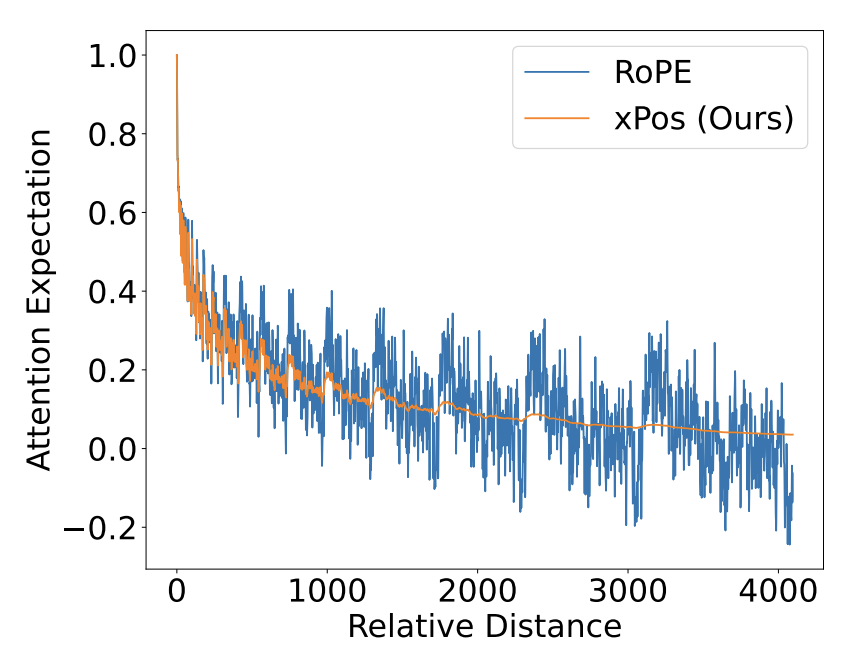
\includegraphics[width=.4\hsize]{exp.png}
            \caption{二つのトークンの相対距離に対するAttentionスコアの期待値}
        \end{figure}
        RoPEでは発振が見られるが、
        提案手法ではそれが抑えられている。
        これにより、Attention Resolutionが増大することが確認された
    \end{frame}
    \begin{frame}{Blockwise Causal Attention}
        出力シーケンスをブロックに分割し、
        ブロックごとに順番にAttention機構に通すことで、
        間接的に離れた距離のトークン同士の情報がAttention行列に
        適用されることが示された
        \begin{figure}[ht]
            \centering
            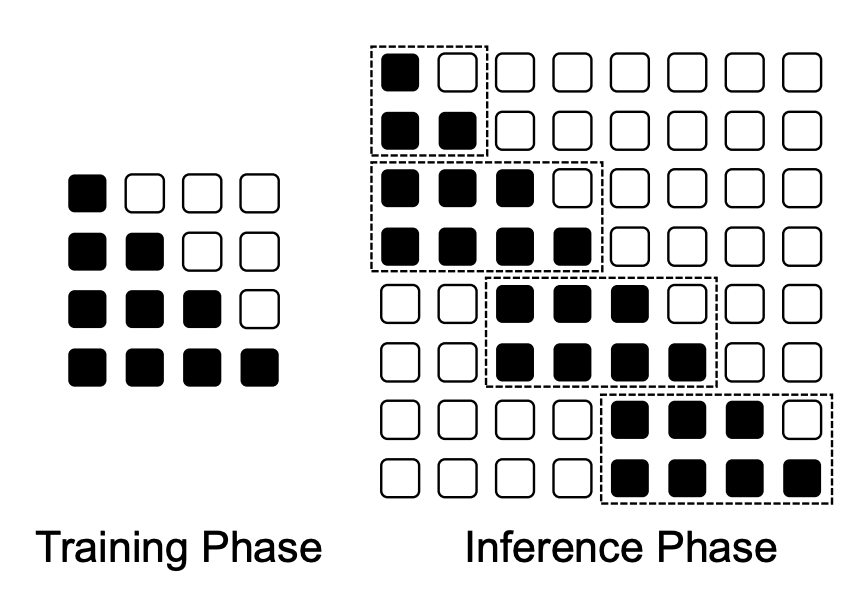
\includegraphics[width=.58\hsize]{block.png}
        \end{figure}
    \end{frame}
    \begin{frame}{実験結果}
        トークン長1024で学習したモデルの、2048トークン、
        4096トークンの入力における外挿能力が検証された
        \begin{figure}[ht]
            \caption{各モデルのPerplexity}
            \centering
            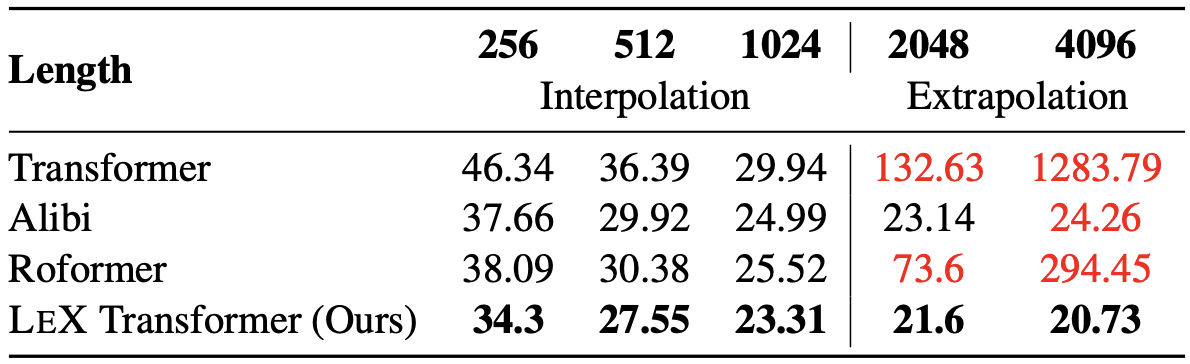
\includegraphics[width=.6\hsize]{lex.png}
        \end{figure}
    \end{frame}
    \begin{frame}{展望}
        理想的なLLMは入出力どちらも外挿可能なアーキテクチャであると考える

        LLMを扱う上で、モデルの再学習は時間・空間計算量の観点で
        大きな障壁となる

        $\rightarrow$\structure{再学習を行わず}に入出力どちらも外挿可能なモデルについて調査・検証を進めていきたい

        \begin{exampleblock}{}
            このような研究を行う上で、事前学習済みのパラメータを用いつつ内部構造に変更を
            加えて検証を行えるモデルが不可欠である
            
            \textcolor[rgb]{0,0.5,0}{
                現状、そのようなモデルが公開されているプラットフォーム等を発見できていない為、
                思い当たる方は是非平田に一報願いたい
            }
        \end{exampleblock}
    \end{frame}
\end{document}